\chapter{\zway enabled Hardware}
\index{Hardware}

\zway is  a complete software solution that is ported on various hardware. In order to run 
it on a certain hardware platform, the following requirements have to be met:

\begin{enumerate}

\item There must be a binary \zway distribution available for this platform. At 
\murl{http://razberry.wave.me/z-way-server} you will find the most recent releases 
of \zway binary distributions for the various platforms supported:
	\begin{enumerate}
	\item Dune HD:  ARM Linux
	\item Alix-x86:  Intel CPU 32 Bit Linux
	\item Contactless
	\item Debian:  Intel CPU 64 Bit Linux Debian distribution
	\item Popp:  For Popp Hub, Mediatek CPU, OpenWRT
	\item Raspberry Pi: for the famous Raspberry Pi, ARM based
	\item Ubuntu: Intel CPU 64 Bit Linux Ubuntu distribution
	\item Windows: For Windows Operating System
	\end{enumerate}
Other platforms may be supported as well by one of these binary distributions.
\item \zwave transceiver connected to the platform containing a \zway license. Currently, 
the 'RaZberry Shield' always comes with an internal license enabled, while the USB Stick called UZB
needs an additional license applied. \zway may also run on platforms with embedded \zwave 
transceivers (such as Popp HUB, Dune HD set-top box), but this requires special 
arrangement with the manufacturer. Please refer to the section \ref{otherhardware} for 
more information.
\end{enumerate}

Please note that \zway will start on a certain platform without having a \zwave transceiver 
or a licensing key. However, in this case is no support for \zwave. Still, this may be a good 
starting point to test the software free of charge. Please refer to the section \ref{apps} 
for possible applications usable without having \zwave enabled.

\zwaveme currents support two basic hardware platforms with \zway licensing:

	\begin{enumerate}
	\item The RaZberry shield board for Raspberry Pi and compatible platforms
	\item The USB Stick 'UZB' for PCs, set-top boxes, NAS, etc.	
	\end{enumerate}
	
\section{RaZberry shield board for Raspberry Pi}
\index{Raspberry Pi}
\index{RaZberry}

\subsection{Compatibility}

The RaZberry shield consists of a single PCBA with a connector to the standard GPIO pin 
header connector of the Raspberry Pi minicomputer. This 25-pin header connector is 
available on all contemporary Raspberry Pi versions, such as:

\begin{itemize}
\itemsep0em
\item Version A
\item Version B
\item Version B+
\item Version 2B
\item Zero
\item Version 3
\end{itemize}

Even if your Raspberry Pi version is not on the list above, there is a very high chance 
that the shield board will work as long as your Pi has the 25-pin GPIO connector. You will 
find more information about the pinout of this 25-pin connector on various websites
\footnote{e.g. http://www.raspberry-pi-geek.de/Magazin/2015/05/Raspberry-Pi-und-Arduino-via-UART-koppeln}.

You can use other pins of the connector for other purposes as long as they do not 
physically conflict with the board.

\subsection{Pinout and options on board}

The RaZberry board use only four pins of this header connector:

\begin{itemize}
\item Gnd
\item VCC (3.3V)
\item Serial TX
\item Serial RX
\end{itemize}

Figure \ref{q1} shows how the board connects to the 25-pin header on a Raspberry Pi 2

\begin{figure}
\begin{center}
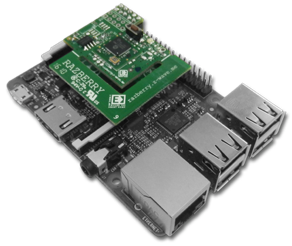
\includegraphics[width=0.4\textwidth]{pngs/cap2/q1.png}
\caption{RazBerry on top of a Raspberry Pi}
\label{q1}
\end{center}
\end{figure}

The board itself offers a few connection options as shown in Figure \ref{q2}:
\begin{enumerate}
\item Raspberry Pi Connector, used GPIO pins 1-10
\item Second open connector, identical to (1)
\item Reset button
\item Open hole for a PigTail antenna. You need to break off the PCBA antenna or unsolder 
resistor S1 to make this work.
\item Pads to solder a uFL connector for external antenna. See 
\murl{https://www.adafruit.com/products/1661} for component details. You need to break 
off the PCBA antenna to make this work.
\item Two LEDs for status information
\end{enumerate}

\begin{figure}
\begin{center}
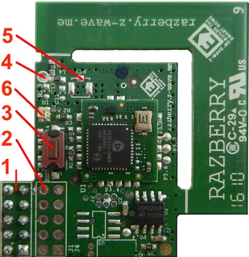
\includegraphics[width=0.4\textwidth]{pngs/cap2/q2.png}
\caption{Components on RaZberry Hardware}
\label{q2}
\end{center}
\end{figure}

The two LEDs are used to indicate the success of the boot-up self-testing and as status 
indicators during normal operation.

\subsection{Boot-Up Self-Test}

When powered up, the two LEDs light up, indicating that the self-testing has started. 
After about two seconds, they are supposed to go off indicating that that self-testing 
has been passed successfully. If they remain lit, this is a clear indication that the 
self-test failed or the device is not booting up. You will need to replace the hardware 
in such a case.

\subsection{LEDs during Operation}

During normal operation, the two LEDs remain turned off except:

\begin{itemize}
\item Green LED will light up when data is transmitted.
\item Red LED will light up when the \zwave transceiver is either in Inclusion or in 
Exclusion mode. Please note that these are special modes of the transceiver that block 
normal data communication with other nodes in the network.
\end{itemize}

\subsection{Frequencies}
\index{Frequency}

The RaZberry shield itself can be tuned into every frequency used by \zwave. However, 
to protect the transceiver and \zwave from high energy emissions on nearby frequencies 
(primarily 4G/LTE cellular radios using the 852 MHz frequency band), an external 
antenna filter is used. This limits the frequency changes to countries that share 
the same antenna filter. Currently, there are three antenna filter versions 
identified by their SKU codes.

\begin{itemize}
\item SKU: ZMEEUZB2 (865…869 MHz):
\begin{itemize}
\item Europe (EU)[default]
\item India (IN)
\item Russia (RU)
\item PR China (CN)
\item RSA (EU)
\item Middle East(EU)
\end{itemize}
\item SKU: ZMEUUZB2 (908 ... 917 MHz):
\begin{itemize}
\item All the Americas except Brazil and Peru (US) [default]
\item Israel (ISL)
\end{itemize}
\item SKU: ZMEAUZB2 (919 ... 921 MHz):
\begin{itemize}
\item Australia/New Zealand/Brazil/Peru/Malaysia (ANZ) [default]
\item Hongkong (HK)
\item Japan/Taiwan (JP)
\item Korea (KR)
\end{itemize}
\end{itemize}

There are two options to change the RaZberry operating frequency:

\begin{enumerate}
\item If you use \zweui, just choose the frontend on \menu{Network > Management} as shown in 
the figure \ref{freqchange}. For more information about this \zweui, please refer to chapter \ref{eui}.
\item There is a shell script available at
\murl{http://www.z-wave.me/fileadmin/download/changezwf.sh} 
Just execute the script with
\begin{quote}
\cmdline{changezwf.sh [COM Port] [US|EU|ANZ|…]}
\end{quote}
\end{enumerate}

\begin{figure}
\begin{center}
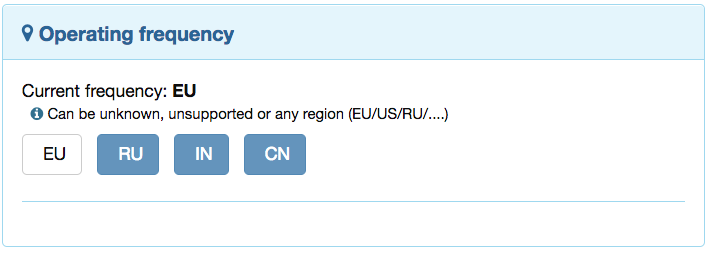
\includegraphics[width=0.6\textwidth]{pngs/cap2/freqchange.png}
\caption{Frequency Change Option in \zweui}
\label{freqchange}
\end{center}
\end{figure}

\subsection{Certifications}
\index{CE}

RaZberry is certified for use in different countries.

\subsubsection {CE / Europe}

RaZberry complies with the new Radio Equipment Directive of the European Union in general 
and the EN 300 220 version 3.1.1 in particular. Full CE declaration can be found in
Annex \ref{annexdeclarations}.
The device also complies with the European ROHs and REACH regulations.

\subsubsection {FCC / North America}
\index{FCC}

The RaZberry shield was successfully tested for FCC. The FCC identifier is

\begin{quote}
\textbf{2AAYUZMEURAZ}.
\end{quote}

\subsubsection {\zwave Plus}

The RaZberry shield is a certified hardware platform and a complete solution according to 
\zwave Plus. Please refer to the certification database 
\murl{http://products.z-wavealliance.org} for more details.


\section{The USB Stick UZB}
\index{UZB}
\index{USB Stick}

The USB Stick 'UZB' allows enabling \zway on various platforms. Figure \ref{uzb} shows the device.

\begin{figure}
\begin{center}
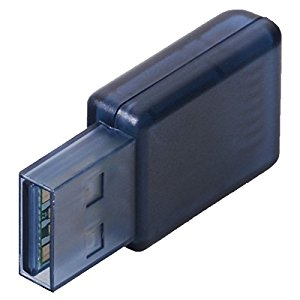
\includegraphics[width=0.3\textwidth]{pngs/cap2/uzb.jpg}
\caption{USB Stick UZB}
\label{uzb}
\end{center}
\end{figure}

It is plugged into a free standard USB port. UNIX-based operating systems will recognize 
the stick and generate a virtual serial device named
\cmdline{/dev/ttyACM0} or \cmdline{/dev/cu.usbmodem} or similar.
Windows will generate one virtual serial port \cmdline{COM XX}.

Once \zway is started, it will connect to the \zwave hardware using this virtual serial device.

The USB stick is very small (presently the smallest \zwave device in the world) and will stick quite 
close to the enclosure of the PC or NAS. This may interfere with the wireless range. 
If you experience problems with the wireless range, please use a standard USB extender 
cable to get the UZB antenna further away from the PC.

In case the UZB is not loaded with a \zway license (the stick is generally sold in two 
versions, one with a license and one without for use with 3rd party software), the 
license can be loaded once \zway is 
up and running. Please use the \zweui as described in Section \ref{eui} to apply 
the license. The license is a simple string that usually comes printed in a scratch 
card. Go to \menu{Network > Controller Info} and click on the button 
\keystroke{License Upgrade}. You will see a dialog as shown in Figure \ref{license}.


\begin{figure}
\begin{center}
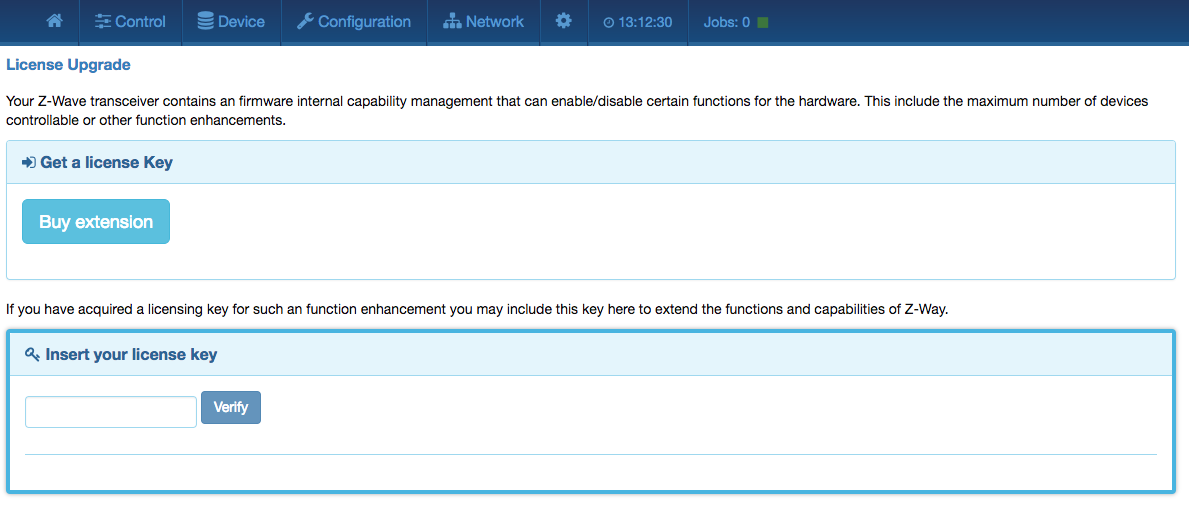
\includegraphics[width=0.9\textwidth]{pngs/cap2/licensefile.png}
\caption{UZB license upgrade}
\label{license}
\end{center}
\end{figure}

The \keystroke{Buy extension} button leads you to instructions about how to extend the 
capabilities of the UZB stick by buying extra licensing files. The input field below 
allows inserting and applying the license key manually. Please note that:

\begin{itemize}
\item You must be connected to the internet to activate the license key.
\item Every license key can only be used once (like scratch cards for prepaid phones).
\item It is possible to apply various license files to the same hardware.
\item The license is stored in the hardware. You can do a complete reinstallation of \zway on 
your platform or connect the UZB to a totally new platform without losing the license. 
However, loosing or damaging the UZB key means loosing the license!
\end{itemize}
It is possible to run multiple UZBs on one single hardware platform or even combine a 
RaZberry shield with a UZB on the same Raspberry Pi. Each piece of hardware will then 
manage its own network of \zwave devices having its own Home ID. However, \zway allows 
using devices of different \zwave networks together. This can be used to use products 
with different frequencies in one controller.

In order to enable a second \zwave transceiver (dedicated onboard, UZB or RaZberry), 
please use the standard user interface as described in Chapter \ref{shui}. 
Go to the app management section and start another instance of the app \app{\zwave Network Access}. 
Choose the new virtual serial device created by the new hardware.

Please note that the standard user interface will support devices from two networks, but 
you need to use the \zweui to manage the second network. The inclusion and exclusion 
functions of the standard user interface will always use the first \zwave network.

\subsection{Boot-Up Self-Test}

On being powered up, the blue LED will light up, indicating that the self-testing has started. 
After about two seconds, the LED goes off, indicating that that self-testing has been 
done successfully. If the LED remains lit, it means that the self-testing has failed or 
the device is not booting up. You will need to replace the hardware in such a scenario.


\subsection{Frequencies}

The \zwave transceiver itself can be tuned into every frequency used by \zwave. However, 
to protect the transceiver and \zwave from high energy emissions on nearby frequencies 
(primarily 4G/LTE cellular radios using the 852 MHz frequency band), an external antenna 
filter is used. This limits the frequency changes to countries that share the same 
antenna filter. As of now, there are three antenna filter versions identified by 
their SKU codes.

\begin{itemize}
\item SKU: ZMEEUZB2 (865…869 MHz):
\begin{itemize}
\item Europe (EU)[default]
\item India (IN)
\item Russia (RU)
\item PR China (CN)
\item RSA (EU)
\item Middle East(EU)
\end{itemize}
\item SKU: ZMEUUZB2 (908 ... 917 MHz):
\begin{itemize}
\item All the Americas except Brazil and Peru (US) [default]
\item Israel (ISL)
\end{itemize}
\item SKU: ZMEAUZB2 (919 ... 921 MHz):
\begin{itemize}
\item Australia/New Zealand/Brazil/Peru/Malaysia (ANZ) [default]
\item Hongkong (HK)
\item Japan/Taiwan (JP)
\item Korea (KR)
\end{itemize}
\end{itemize}

There are two options to change the UZB operating frequency:

\begin{enumerate}
\item If you use \zweui, just choose the frontend on \menu{Network > Management} as shown in the figure.
\ref{freqchange}. For more information about this \zweui, please refer to Chapter \ref{eui}.
\item There is a shell script available at 

\murl{http://www.z-wave.me/fileadmin/download/changezwf.sh} 
Just execute the script with

\begin{quote}
\cmdline{changezwf.sh [COM Port] [US|EU|ANZ|…]}
\end{quote}

\end{enumerate}

\subsection{Certifications}

The UZB is certified for use in different countries.

\subsubsection {CE / Europe}

The UZB complies with the new Radio Equipment Directive of the European Union in general 
and the EN 300 220 version 3.1.1 in particular. Full CE declaration can be found in
Annex \ref{annexdeclarations}.
The device also complies with the European ROHS and REACH regulations.

\subsubsection {FCC / North America}

The UZB stick shield was successfully tested for FCC. The FCC identifier is

\begin{quote}
\textbf{2AAYUZMEUUZB}.
\end{quote}

\subsubsection {\zwave Plus}

The UZB USB stick is a certified hardware platform and a complete solution according to 
\zwave Plus. Please refer to the certification database 
\murl{http://products.z-wavealliance.org} for more details.

\section {Other hardware platforms}
\label{otherhardware}

It is possible to port \zway to other hardware platforms beyond what is supported by 
binary distributions. Before contacting the \zwaveme team, you can check if your platform 
meets the requirements for \zway to run on. The general requirements are:
\begin{itemize}
\item min. 200 MHz CPU clock speed,
\item CPU architecture based on ARM, Intel or MIPS, as well as a GNU-based development tool chain,
\item min. 16 MB Flash memory and 12 MB RAM,
\item Operating system supports POSIX-compatible API.
\end{itemize}

There is a simple test to check if certain hardware on a platform is capable of running \zway.
Follow the instructions given on

\begin{quote}
\textbf{http://razberry.z-wave.me/index.php?id=28}.
\end{quote}

Only after you have double-checked that a binary distribution runs on your system or that 
the compatibility test has been passed, you may want to contact the \zwaveme team for 
further discussions about porting and licensing fees.
